\begin{enumerate}
    \item FreeRTOS is a form of \href{https://en.wikipedia.org/wiki/Cooperative_multitasking}{co-operative multitasking}. Basically the microprocessor (STM32) will switch between the tasks as each one finishes its processing
    \item Follow steps 1-6 of the LED Blink tutorial to set up a new CubeMX project
    \item Now enable UART (same as last tutorial) but with a baud rate of 115200 Bits/s
    \begin{enumerate}
        \item No need to enable the global interrupt for this tutorial
    \end{enumerate}
    \item Now, scroll down to the "Middleware and Software Packs" drop down menu and click on "FreeRTOS"
    \begin{enumerate}
        \item Select "CMSIS\_V2" on the "Interface" drop down menu \vspace{0.25cm}\\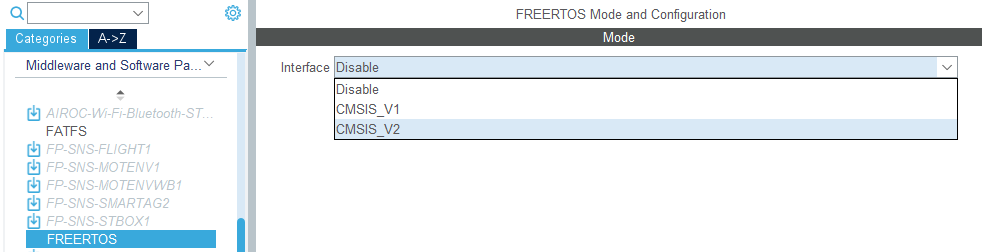
\includegraphics[width=0.9\columnwidth]{FreeRTOS 1.png}
    \end{enumerate}
    \item Go to the "Tasks and Queues" tab and click the "Add" button
    \begin{enumerate}
        \item Here is where we will make two FreeRTOS tasks to add (append), and remove from a queue
    \end{enumerate}
    \item Here are the settings you need to change for the first task:
    \begin{enumerate}
        \item Call the first task "queueAppendTask"
        \item Set it's priority to "osPriorityLow"
        \item Leave Stack Size (Words) as 128
        \item Change the name of the entry function to "StartQueueAppendTask"
        \item Leave Code Generation Option as "Default"
        \item Leave Parameter as "NULL"
        \item Leave Allocation as "Dynamic"
    \end{enumerate}
    \item Now, create another task according to these settings:
    \begin{enumerate}
        \item Call the first task "queueRemoveTask"
        \item Set it's priority to "osPriorityLow"
        \item Leave Stack Size (Words) as 128
        \item Change the name of the entry function to "StartQueueRemoveTask"
        \item Leave Code Generation Option as "Default"
        \item Leave Parameter as "NULL"
        \item Leave Allocation as "Dynamic"
    \end{enumerate}
    \item Next, we want to make the queue that these two tasks will use to send and receive messages
    \item Click "Add" under the Queues section
    \item Here are the queue settings:
    \begin{enumerate}
        \item Call the queue "coolQueue"
        \item Set the queue size to 8
        \item Set the item size to "uint16\_t"
        \item Set the allocation to "Dynamic"
    \end{enumerate}
    \item Now, go to the "Project manager" tab and call the project "HAL\_FreeRTOS\_Tutorial", set the project file location and set the Toolchain/IDE to STM32CubeIDE
    \item Click generate code
    \item The functions you will need to use in this tutorial come from the CMSIS-RTOS2 (CMSIS\_V2) version of FreeRTOS
    \begin{enumerate}
        \item You can find these functions in the "Middlewares" folder of our project. CubeMX automatically generated these files when we enabled the CMSIS\_V2 FreeRTOS functionality
    \end{enumerate}
    \item Here's a hyperlink to some documentation on these functions: \href{https://www.keil.com/pack/doc/CMSIS_Dev/RTOS2/html/group__CMSIS__RTOS__Message.html}{CMSIS\_V2 FreeRTOS Queue Functions}
    \item In main.c, we want to add (append) data to the queue using the StartQueueAppendTask() and remove data from the queue using StartQueueRemoveTask().
    \item Use the following code inside StartQueueAppendTask(). We want to increment dataSend inside the infinite loop and append it to the queue
    \begin{lstlisting}[style=CStyle]
uint16_t dataSend = 0;
const uint16_t MAX = 100;
    \end{lstlisting}
    \item Once the count reaches a max of 100 we want to reset the data sent value to 0.
    \item Use the following code inside StartQueueRemoveTask():
    \begin{lstlisting}[style=CStyle]
uint16_t dataReceived = 0;
char new_char[5];
    \end{lstlisting}
    \item In StartQueueRemoveTask(), you want to remove the data from the queue and transmit the data you get to your COM port so PuTTY can view it. Use the HAL\_UART\_Transmit() function to transmit the message!
    \begin{enumerate}
        \item Hint: You'll need to use the following code to convert the data to the correct type to transmit via UART!
    \begin{lstlisting}[style=CStyle]
snprintf(new_char,"%d\r\n",dataReceived);
    \end{lstlisting}
    \end{enumerate}
    \item At the end of the FreeRTOS tasks, StartQueueAppendTask() and StartQueueRemoveTask() you'll need to use osDelay() to guarantee the function has enough time to fully execute its processing
    \begin{enumerate}
        \item Pass the function the following code as its parameter converting the number you enter in milliseconds to the equivalent number of ticks:
    \begin{lstlisting}[style=CStyle]
pdMS_TO_TICKS(100)
    \end{lstlisting}
    \end{enumerate}
    \item Once you run PuTTY with the correct baud rate, you'll know if your code works if you get the output that counts to 99 then resets to 0 and continues counting!
\end{enumerate}